\documentclass{article}
\usepackage{import}
\subimport{../}{preamble}
\begin{document}

\section{Scanning Capacitive AFM Tip Alignment}
\label{sec:tip_alignment}

A significant challenge when attempting to recreate a plasmonic dimer using opposing AFM probes is the alignment of tips with the focussed laser spot in a symmetric tip-to-tip configuration. This capability is necessary to permit the majority of dual tip experiments and forms the first step to measuring the dynamical physical response of plasmonic tip dimer systems. For successful experiments the tolerance on the tip-to-tip alignment is less than \orderof{$R_{\mathrm{tip}}$}. Aligning tips using CCD imaging is limited by diffraction and therefore unsuitable. Initially this problem was solved using a non-linear capacitive alignment technique that required locking into the third harmonic of the driving signal \cite{savage2011}. Whilst functional in simpler systems, the technique was limited in its accuracy by the small pA level currents in the third harmonic mode and the extensive filtering and lock-in techniques required to measure these. A simpler approach is to simply use the AFM module optics to measure the oscillating cantilever deflection. This is more widely known as scanning capacitance mode AFM (SC-AFM) or \gls{scm}, and has been used in the past to measure the dopant levels in semiconducting substrates \cite{matey1985scanning, bugg1988scanning, huang1995quantitative, kopanski1996scanning, girard2001electrostatic}. By utilising optical detection over direct electronic measurements tip alignment becomes segregated from the microscope electronic d.c.\ measurement circuitry and issues are no longer caused by noise leaking into the a.c.\ electronics.

\subsection{Mechanism for Alignment of Two Opposing Tips}

\begin{figure}[bt]
\centering
\fontsize{10pt}{1em}\selectfont
\def\svgwidth{0.65\textwidth}
\subimport{./figures/}{tip_alignment_diagram.pdf_tex}
\caption[Diagram of tip alignment parameters]{\textbf{Diagram of tip alignment parameters.} The position of one tip relative to the other is detected using a resonant scanning capacitance AFM technique. The gap is biased with an oscillating voltage to induce a resonant vibration of one of the AFM cantilevers. The amplitude of oscillation is sensitive to the gap size $d$ and the area of overlap $A_{ov}$ between tip features of characteristic size $R$. For sharp tips $R$ is the apex radius whereas for nanostructured tips $R$ is considered to be the feature size.}
\label{fig:tip_alignment_diagram}
\end{figure}

% Describing the initial EoM of the full system
To a first approximation the metallic tips can be ignored and only the capacitive interaction between planar cantilevers is considered. Cantilevers are separated by a distance $d(t) = z_1(t) - z_2(t)$ and coupled via the $z$-components of the long range, attractive, electrostatic driving force $F_{EL}^z$ and short range  Van da Waals and repulsive tip-tip interaction forces $F_{TT}^z$. Each cantilever has an associated spring constant $k_{0i}^z$, mass $m_i$ and resonant frequency of oscillation $\omega_{0i} = \sqrt{k_{0i}/m_i}$. When vibrated, cantilevers oscillate around an equilibrium position $z_{0i}$. The equilibrium separation between tips is then denoted by $d_0 = z_{01} - z_{02}$.

The equation describing motion in the $z$-axis of the two parallel cantilevers, denoted by $i=1,2$, of spring constant $k_i^z=k_{0i}^z+k_{TT}^z$, coefficient of damping $\beta_i^z=\beta_{0i}^z+\beta_{TT}^z$ and mass $m_i$, is given by,
\begin{equation}
	m_i\frac{d^2z_i}{dt^2}+\beta_i^z\frac{dz_i}{dt}+k_i^z\left(z_i-z_{0i}\right)=\pm\left(F_{EL}^z+F_{TT}^z\right),
\end{equation}
where the sign of the force is positive for one tip and negative for the other.
% Simplifications
Assuming that alignment takes place at long range, tip-tip interactions can be ignored, therefore $F_{TT}^z = 0$ and $\beta_{TT}^{z} = k_{TT}^{z} = 0$. The system is further simplified by assuming that one cantilever remains stationary by being stiff (tapping mode tip with $k\approx\SI{40}{\newton\per\metre}$)%
\footnote{This is based on data sheet values of almost all tapping mode tips.}
and always being off resonance ($\omega_{01} \neq \omega_{02}$). This is usually satisfied in experiments where a stiff cantilever is required such that the optical probe is incident on the same sample area whilst under force. The apex separation is then restricted to $d=z_1$ with an equilibrium separation $d_0 = z_{01}$. Under these conditions the motion reduces to that of a single tip,
\begin{equation}
	m_1\frac{d^2z_1}{dt^2}+\beta_1^z\frac{dz_1}{dt}+k_1^z\left(z_1-d_0\right) = F_{EL}^z(z_1, t).
	\label{eq:simple_eom}
\end{equation}
This equation now describes the whole system rather than each individual tip with the main reference point between tips being the equilibrium separation $d_0$.

% Description of the electrostatic force
The remaining capacitive driving force exerted between tips is purely electrostatic and of the form,
\begin{equation} F_{EL}^z(V,z) = \frac{1}{2} \frac{\partial C(z)}{\partial z} V^2(t), \end{equation}
where $C(z)$ is the capacitance between the tips at a distance $z$ and $V(t)$ is the potential difference between tips. Under a parallel plate capacitor model the capacitance is $C(z) = {(\varepsilon_0 A_{ov}}/{z}) + C_{bk}$ for plates with $A_{ov}$ area of overlap at a separation $z$, including a stray capacitance $C_{bk}$. Applying a harmonic driving force at a frequency $\omega_s$, described by $V(t)=V_0 \cos(\omega_s t)$, results in a nonlinear driving force, given by,
\begin{equation}
	F_{EL}^z(z_1,t) = \left(\frac{-\varepsilon_0 A_{ov} V_0^2}{4z_1^2}\right)\left[1+\cos(\omega_pt)\right],
	\label{eq:driving_force}
\end{equation}
where $\omega_p = 2\omega_s$ is the cantilever pump frequency.
% Deriving the final EoM of the simplified system
Substituting \eqref{eq:driving_force} into \eqref{eq:simple_eom} gives the simplified equation of motion for the dual-tip system,
\begin{equation}
m_1 \frac{d^2z_1}{dt^2} + \beta_{01}^z \frac{dz_1}{dt} + k_{01}^z (z_1-d_0) = \left( \frac{-\varepsilon_0 A_{ov} V_0^2}{4z_1^2}\right)\left[1+\cos(\omega_pt)\right].
\label{eq:final_eom}
\end{equation}
Driving at a pump frequency close to the cantilever resonance ($\omega_p \approx \omega_{01}$) leads to a resonant oscillation between tips. For small oscillations around $d_0$, \eqref{eq:final_eom} can be Taylor expanded to first order into the form of the damped Mathieu equation%
\footnote{Damped Mathieu equation: $\ddot{z} + 2\kappa\dot{z} + [a - 2q\cos(2t)]z = 0$}
with an approximate solution%,
\footnote{Full derivation available in the appendix.}
\begin{equation}
z_1 \approx d_0 - \left|z_{1}^{off}\right| - z_{m1}\cos(\omega_pt+\varphi_1)
\label{eq:tip_oscillation}
\end{equation}
where
\begin{subequations}
\begin{align}
z_1^{off} &\approx %
\frac{ \varepsilon_0 A_{ov} V_0^2 }{ 4d_0^2 \langle k_{e1}^z \rangle }, \\
%
z_{m1} &\approx %
\frac{ \varepsilon_0 A_{ov} V_0^2 }%
{ 4d_0^2 \sqrt{ (\langle k_{e1}^z \rangle - m_1\omega_p^2)^2 + (\beta_{01}^z\omega_p)^2  } }, \label{eq:tip_amp} \\
%
\varphi_1 &\approx \tan^{-1}\left(\frac{\beta_{01}^{z}\omega_{p}}{\langle k_{e1}^{z} \rangle -m_{1}\omega_{p}^{2}}\right), \label{eq:tip_phase}
\end{align}
\end{subequations}
in which $\langle k_{e1}^z \rangle$ is the effective spring constant of the system, $\langle k_{e1}^{z} \rangle = k_{01}^z - {\varepsilon_0 A_{ov} V_0^2}/{2d_0^3}$, taking into account the time-averaged electrostatic interaction. From \eqref{eq:tip_amp} and \eqref{eq:tip_phase} it can be seen that both the oscillation amplitude and phase relative to the driving signal vary with the equilibrium separation $d_0$.

Although the model is for two parallel plates, it becomes applicable to tips in a dimer configuration once the separation is sufficiently low that the tip-to-tip capacitance dominates over all other capacitive contributions (such as the cantilever or tip facet interactions). In this regime, if the tips stray out of alignment the tip-to-tip distance increases and the capacitance decreases, reducing the tip oscillation amplitude and the phase, hence tips are aligned when both the amplitude and phase are maximised. Both these properties are readily measurable using optical cantilever deflection in the AFM module.

% Previous Electronic Alignment Methods without AFM Measurement
Whilst optical detection gives a better signal-to-noise and measures at higher bandwidths, it should be noted that the capacitive model was originally developed to show that a $3\omega_s$ current signal can be used to align tips \cite{savage2011}. By driving the system with $\omega_p \approx \omega_{01}$, a mechanical parametric resonance is excited at $2\omega_{01}$ (otherwise only the fundamental is excited with resonant driving) and the current through the tip junction is given by,
\begin{subequations}
\begin{align}
I(\omega_{s}) & \approx \omega_{s}C_{0}V_{0} \left(1+\frac{|z_{off}|}{d_{0}}+\frac{z_{m1}}{2d_{0}}\e^{i\varphi_1}+\frac{C_{bk}}{C_{0}}\right)\e^{i\frac{\pi}{2}},\\
%
I(\omega_{p}+\omega_{s}) & \approx \frac{\left(\omega_{p}+\omega_{s}\right)C_{0}V_{0}z_{m1}}{2d_{0}} \e^{i\left(\varphi_1 + \frac{\pi}{2}\right)},
\label{eq:3rd_harmonic_current}
\end{align}
\end{subequations}
where $C_0 = \varepsilon_0 A^{ov} / d_0$ and $z_{off}$ is an additional offset due to $F_{EL}^z \propto V^2$. Non-linear oscillations in the tip capacitance result in parametric frequency mixing in the electronics with resulting signals at the sum and difference frequencies, $\omega_{p}+\omega_{s}=3\omega_{s}$ and $\omega_{p}-\omega_{s}=\omega_{s}$ respectively. The signal at $3\omega_{s}$ is background-free, as shown in \eqref{eq:3rd_harmonic_current}, and once again depends only on $z_{m1}$ and $d_{0}$. However, currents are \orderof{pA} for acceptable driving voltages, therefore alignment only works over shorter ranges, and requires larger voltages to further boost the oscillation amplitude and low-noise detection electronics. Optical detection is advantageous as small oscillations at lower voltages are easily detectable, which protects the samples from damage caused by tapping between tips once the gap is small.

\subsection{Numerical Modelling and Experimental Measurements of Scanning Capacitance Tip Alignment}

\subsubsection{Numerical Modelling of Tip Alignment}

Theoretical curves for the system response based on \eqref{eq:final_eom} for a typically used contact/tapping mode AFM probe dimer are solved numerically using an \gls{ode} solver.%
\footnote{ODE in Numpy/Python}
Results are intended to \textit{qualitatively} demonstrate the alignment technique.
% Summary of parameters
The following table summarises the parameters of the model for each tip:
\begin{table}[H]
\begin{center}
\begin{tabular}{c | c | c}
\hline
& \textbf{Tip 1} & \textbf{Tip 2} \\
\hline                 
$k_0$ (N/m) & 0.2 & 40 \\
$\omega_0$ (kHz) & $2\pi.13$ & $2\pi.300$ \\
$\Delta\omega$ (Hz) & $2\pi.200$ & $2\pi.200$ \\
$r$ (nm) & 20 & 20 \\
\hline 
\end{tabular}
\end{center}
\caption[Tip parameters used in numerical calculations]{\textbf{Tip parameters used in numerical calculations.} The dimer is assumed to comprise of a dynamic contact mode AFM cantilever (tip 1) and a fixed tapping mode cantilever (tip 2).}
\vspace{-10pt}
\end{table}
The plate area is assumed to be $\pi r^2$ where $r$ is the radius of the tip. This is estimated to be $r=\SI{20}{nm}$ based upon standard tip apex dimensions. Changing this value does not change the overall qualitative shape of the data. The mass of each tip is calculated from the resonance using $m_i = k_{0i}/\omega_{0i}^2$. The damping coefficient of each tip is given by $\beta_{0i} = 2m\delta_i$ where $\delta_i = \omega_{0i}/2Q_i$ and $Q_i = \omega_{0i}/\Delta\omega$ (a quantity which is verifiable by experiment). Only the damping coefficient of the vibrating tip matters at any given time due to the large difference in resonant frequencies. To maximise the detected response the system is studied around the resonance of the soft cantilever.
% The system model
The system spring constant is given by,
\begin{equation}
	k_0 = \left( k_{01}^{-1} + k_{02}^{-1} \right)^{-1},
\end{equation}
and the system mass is given similarly by,
\begin{equation}
	m = \left( m_1^{-1} + m_2^{-1} \right)^{-1}.
\end{equation}
%The damping coefficient of the system is calculated using,
%\begin{equation}
%\beta = 2m_1\delta_1 \left( 1 + \frac{r_1^2}{z} + \frac{(20\e^{-6})^2}{z(2-20\e^{-6})} \right),
%\end{equation}
%where $\delta = \Delta\omega/2$.

% Tip forces in the model
The forces acting on the tip are described by a capacitive driving force, described by \eqref{eq:driving_force}, and an interaction force. The interaction force is described by,
\begin{equation}
	F_i^z(z) =
	\begin{dcases}
	-\frac{H r_1}{6(a+z_c)^2}, & \text{if } z_c + a > a_0 \\
	-\frac{H r_1}{6a_0^2} + \frac{4E\sqrt{r_1}}{3 - 3v^2} (a_0-a-z_c)^{\frac{3}{2}}, & \text{otherwise}
	\end{dcases}
	\label{eq:tapping_force}
\end{equation}
where $z_c$ is the equilibrium position, $a$ is the amplitude of the oscillation, $a_0$ is the equilibrium separation and $H$ is the Hamaker constant \cite{tamayo1996deformation, garcia1999attractive, san2002unifying, lee2002nonlinear}. The capacitive driving force depends only on the time-averaged tip separation whilst the interaction force depends on the oscillation amplitude of the tip around its equilibrium position compared with the gap separation since this eventually leads to tapping on the opposite tip.

% Temporal response calculation
The ODE algorithm computes the change in the cantilever position and velocity in time using their respective differentials,
\begin{align}
	\dot{z}_+ &= \dot{z}_-, \\
	\ddot{z}_+ &= -m^{-1}\left[\beta_1^z\dot{z}_- - k_0^zz_- + F_{EL}^z(t) + F_i^z(z_-)\right],
\end{align}
where $F_{EL}^z(t)$ is the capacitive driving force described in \eqref{eq:driving_force}, $F_i^z(z)$ is the interaction described in \eqref{eq:tapping_force}. The tip motion in time is solved, subject to stationary initial conditions, for 100 AFM oscillation periods. The steady state harmonic properties of the waveform are extracted using a sinusoidal fit to the last 50 periods, when behaviour has stabilised.

The modelled frequency response is determined by driving a spatially fixed tip dimer, separated by \SI{100}{nm}, with a \SI{10}{V} driving signal across a range of frequencies around $\omega_s = \omega_{01}/2 = 2\pi.\SI{13}{kHz}/2$. The intertip separation is then varied while driving on resonance at various voltages to find the separation response.

\subsubsection{Experimental Measurements using Scanning Capacitance Microscopy}

% Experimental acquisition
Experimental measurements of capacitive tapping mode tip interaction use the AFM optics on the microscope and monitor the position of the tip through the motion of the reflected laser beam. The backside of the softer cantilever of the pair is illuminated by the \SI{633}{nm} laser beam. By resonantly driving an AFM tip electronically its oscillation generates a signal $A\cos(\omega_p t + \phi)$ along one of the axes on the PSD. Lock-in detection is used in the software to remove noise and add phase sensitivity to signal measurements by referencing the oscillation to the driving signal. The NIDAQ device simultaneously acquires both PSD signals in each direction along with the driving signal from the function generator output. The second harmonic of the driving frequency, $\omega_p$ is locked-in using the reference periodicity. The phase difference $\phi$ is then measured relative to the reference phase.%
%\footnote{The software lock-in procedure is detailed in depth in the appendices.}

Experimental measurements are performed on a tip dimer consisting of a \SI{13}{kHz}, \SI{0.2}{N.m^{-1}} soft Au contact-mode AFM cantilever and a \SI{300}{kHz}, \SI{40}{N.m^{-1}} stationary Au tapping mode AFM cantilever. The resonance frequency of the softer cantilever is determined prior to tip alignment at long range by scanning the driving signal frequency and measuring the cantilever response. The separation response is probed by aligning the soft tip to the position of maximum amplitude by laterally scanning the $xy$ plane opposite the stiff tip. The soft tip is approached towards the stationary tip along the $z$ axis and the cantilever response is measured. The rate of approach varies between 0.5--\SI{2}{nm} per step depending on how far apart tips are separated. The amplitude is monitored in real time and the tip is retracted once the signatures of tapping are detected. Quick retraction is necessary as tapping with a soft cantilever is unstable to effects such as snap-in and short-range attractive forces. There is also a high chance of damaging the metallic tip coating during contact. Judgement of the retraction point is subjective since the point of snap-in cannot be predicted but preserves the tip for multiple cycles. This approach-reaction cycle is repeated many times with a continuously reducing voltage until tapping is difficult to achieve without the oscillation immediately becoming unstable. This occurs once driving with less than 5--\SI{6}{V}.

\subsubsection{Comparison between Numerical Modelling and Experimental Scanning Measurements}

\begin{figure}[bt]
\centering
\begin{tikzpicture}
\node [below left] at (0,0) {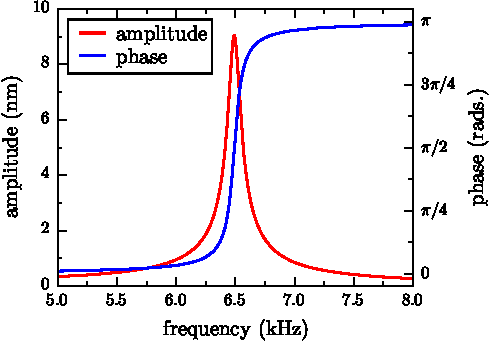
\includegraphics{figures/afm_theory_frequency_response}};
\node [below right] at (0,0) {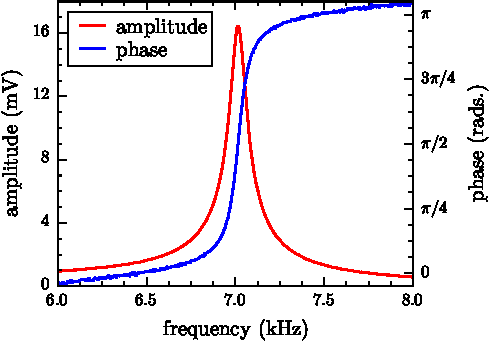
\includegraphics{figures/exp_resonance_scan}};
\node [left] at (-8,-0.2) {\textbf{a}};
\node [right] at (0,-0.2) {\textbf{b}};
\end{tikzpicture}
\caption[Theoretical and experimental frequency response showing the amplitude and phase of a standard opposing AFM tip system]{\textbf{Theoretical and experimental frequency response showing the amplitude and phase of a standard opposing AFM tip system.} The modelled tip junction (a) consists of a \SI{13}{kHz}, \SI{0.2}{N.m^{-1}} soft tip and a \SI{300}{kHz}, \SI{40}{N.m^{-1}} stationary tip, held at \SI{10}{V} with a \SI{100}{nm} intertip separation. Experimental cantilevers (b) are a \SI{13}{kHz}, \SI{0.2}{N.m^{-1}} BudgetSensors ContGB Au tip and a \SI{300}{kHz}, \SI{40}{N.m^{-1}} BudgetSensors TapGB Au tip, separated by $\sim$\SI{1}{\micro\metre} and driven at \SI{15}{V}.}
\label{fig:frequency_response}
\end{figure}

% Frequency response
\autoref{fig:frequency_response}a shows the calculated frequency response for a dimer comprised of a stiff, tapping mode cantilever and a softer contact mode cantilever. From this the cantilever resonance can be clearly seen. The amplitude line shape matches the expected Lorentzian response of a damped resonator and oscillations transition between in-phase oscillation when driving at lower frequencies and anti-phase oscillation at higher frequencies. This is standard resonator behaviour as expected.
The measured frequency response of a capacitively-driven contact mode AFM cantilever (\autoref{fig:frequency_response}b) agrees well with the modelled response. The resonance frequency is higher than expected due to the tolerance range of real AFM cantilevers. One noticeable difference is the linear gradient superimposed onto the phase response. This stems from time lags during acquisition which give a linear phase offset with increasing frequency. % does this need explaining more?

\begin{figure}[bt]
\centering
\begin{tikzpicture}
\node [below left] at (0,0) {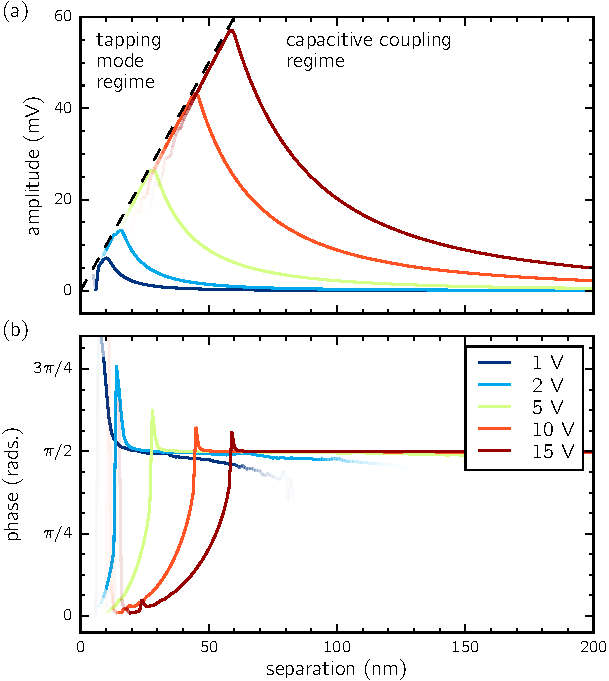
\includegraphics{figures/afm_theory_separation_response}};
\node [below right] at (0,0) {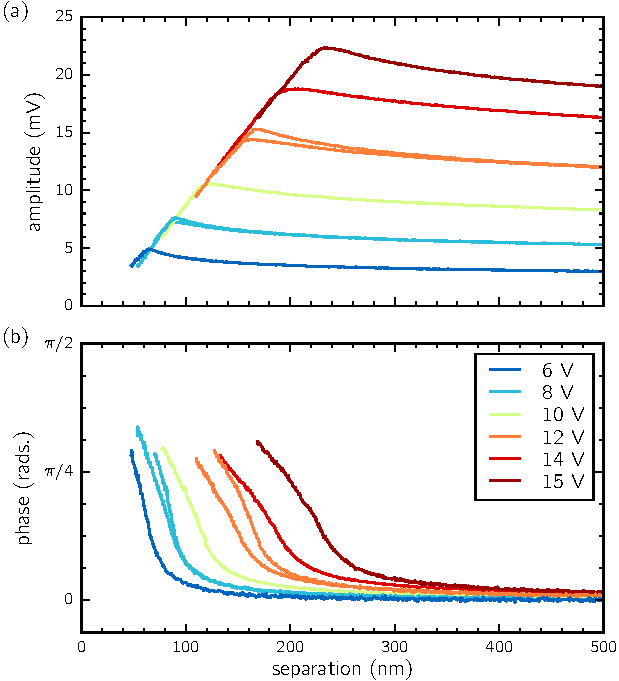
\includegraphics{figures/exp_separation_response}};
\node [below right] at (-4,-1)
{\fontsize{8pt}{1em}\selectfont \def\svgwidth{0.2\textwidth}
\subimport{figures/}{tip_separation_response_diagram.pdf_tex}};
\end{tikzpicture}
{\caption[Theoretical and experimental separation response showing the amplitude and phase of a standard opposing AFM tip system]{\textbf{Theoretical and experimental separation response showing the amplitude and phase of a standard opposing AFM tip system.} The modelled tip junction (a, b) consists of a \SI{13}{kHz}, \SI{0.2}{N.m^{-1}} soft tip and a \SI{300}{kHz}, \SI{40}{N.m^{-1}} stationary tip. The voltage across the modelled tip junction is varied while on resonance ($\omega_s = 2\pi.\SI{6.5}{kHz}$). The amplitude increases as the intertip separation is reduced. The dashed line shows the point at which the oscillation amplitude is equal to the separation. For separations below this limit, the hard surface restricts the amplitude to the gap between tips. A diagram of this is shown as an inset. Experimental cantilevers (c, d) are a \SI{13}{kHz}, \SI{0.2}{N.m^{-1}} BudgetSensors ContGB Au tip and a \SI{300}{kHz}, \SI{40}{N.m^{-1}} BudgetSensors TapGB Au tip. The same vibrating tip is approached and retracted with the voltage reduced between each approach cycle. The amplitude increases as the intertip separation is reduced until oscillation becomes restricted by the gap width.}
\label{fig:separation_response}}
\end{figure}

% Separation response
The calculated separation response for the same contact/tapping-mode tip dimer is shown in \autoref{fig:separation_response}a. As the separation decreases the capacitance between tips increases and resonant oscillation is amplified. This amplification occurs until the amplitude is equal to the separation, at which point the system transitions into the tapping mode of AFM imaging. This is shown by the linear relationship of unity gradient between amplitude and separation, regardless of voltage. In this regime the oscillation is restricted by the gap width between tips, which limits the maximum possible amplitude.
Calculations indicate that phase contrast only occurs once the oscillating tip comes into close proximity with the other tip. This onset of phase contrast occurs close to the point of maximum amplitude just before tapping. The phase is therefore a good indicator of the alignment between tips. Tips can be considered to be aligned once the centres of both the amplitude and phase overlap in a plane perpendicular to the two tips. The accuracy of these solutions becomes limited when the separation is reduced well into the tapping mode regime as the oscillation is difficult to sustain and surface (interfacial) forces begin to dominate, leading to the snap-in effect.%
\footnote{Snap-in, also known as snap-to-contact, is an AFM phenomenon described in a later chapter as a result of capillary forces from a water meniscus in the gap.}
This instability is seen by the deviation of the amplitude from its linear decrease in the tapping regime followed by its rapid decay.

\autoref{fig:separation_response}b shows the corresponding experimental curve to the numerically calculated separation response. The expected capacitive increase in amplitude followed by a linear tapping mode regime is qualitatively found in the experimental data. Differences from numerical calculations, such as the less drastic capacitive amplitude increase, are likely due to the large extended shape of the tip and cantilever not taken into account in the simple parallel plate model. The linear decrease is also less steep suggesting that only the upper region of the modelled curve is visible. The amplitude instabilities found in the calculations at small separations are also found in the experimental data. Repeat approaches after such an instability show different peak amplitudes with the differences attributed to misalignment after contact, changes in tip morphology or surface modification. Interestingly, the discontinuous reduction in the phase is not experimentally observed. This means that either the separation was not reduced enough for this to occur before retraction or the model is not completely correct. Both statements are equally likely due to the simplicity of the model used. Overall the cantilever behaviour qualitatively matches many of the trends predicted using a simple mathematical model solved using an ODE solver. As expected, the separation sensitivity of this technique makes it highly suited for tip alignment.

Another application for capacitive driving, demonstrated by \figurename~\ref{fig:separation_response}, is to use the long range interaction to lock the positions of the tips relative to each other, using the separation-dependent amplitude response as a feedback mechanism in a PID loop.%
\footnote{Proportional-integral-differential (PID) control loops are a form of feedback mechanism for stabilising a value at a preset target.}
Dynamic positioning and alignment between two tips can then be locked and maintained throughout an experiment to account for fluctuations due to either mechanical or thermal drift. Smaller separations can be locked by decreasing the voltage to reduce the amplitude up until the point at which the second harmonic signal becomes difficult to detect. The onset of tapping also limits the minimum achievable separation as the tip must remain oscillating. This technique could potentially become more useful if a stable plasmonic gap size is required for a long time whilst the contents or properties of the gap are modified.

\FloatBarrier
\subsection{Experimental Alignment of Tips using Scanning Capacitance AFM}

% The alignment procedure
By mapping the lateral amplitude and phase variations of the cantilever deflection on resonance, two opposing tips can be experimentally aligned. Alignment is carried out on resonance by laterally scanning the oscillating, soft cantilever tip over the stationary tip whilst reducing the separation. The location of the opposite tip is then determined by the position of maximum amplitude and phase. To prevent tip collisions due to entering the tapping regime, the voltage is reduced along with the separation. This allows only the minimum required signal for positional analysis. Unlike the phase, the amplitude signal varies smoothly over a longer range. As the intertip separation decreases, the amplitude centroid converges on the position of the opposing tip apex and the phase begins to increase and form a sharp peak.  By iteratively following the lateral position of maximum amplitude the tips can be brought into alignment. This procedure is advantageous as it operates at long range in the non-contact regime, prior to the tapping mode regime.

\begin{figure}[bt]
\centering
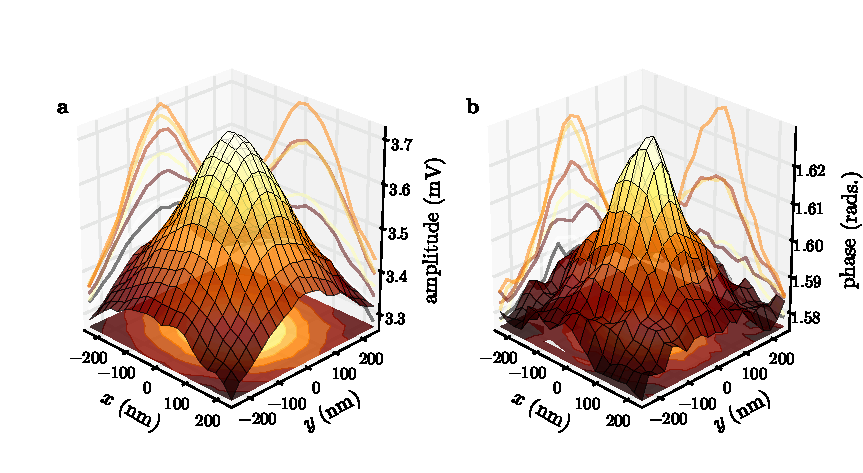
\includegraphics[clip=true, trim=27 19 0 33]{figures/alignment_scan}
\caption[Alignment scan of a soft Au AFM tip scanned laterally over a stiff Au AFM tip]{\textbf{Alignment scan of a soft Au AFM tip scanned laterally over a stiff Au AFM tip.} The soft tip is oscillating at \SI{13}{kHz} (BudgetSensors ContGB) while the \SI{300}{kHz} Au tip (BudgetSensors TapGB) remains static. Tips are separated by $\sim$\SI{50}{nm} and driven at \SI{8}{V}, remaining in the capacitively coupled regime. Strong peaks are seen in both the amplitude and the phase of the soft cantilever oscillation. The tips are aligned in a tip-to-tip configuration when both signals are maximised.}
\label{fig:alignment_scan} 
\end{figure}

\figurename~\ref{fig:alignment_scan} shows a typical alignment scan at close range with peaks in both the amplitude and phase. At this point during the procedure the tips are considered to be well aligned. Tips are then brought into alignment by identifying the position of the peaks. Since the tips are only symmetric along one axis, long range capacitive coupling is inhomogeneous and skewed until the distance between tips is small enough that the tip-to-tip capacitance dominates interactions. Gaussian fitting is therefore potentially inaccurate in determining the peak location. Calculating the centroid from discrete image moments, given by \eqref{eq:image_moments} and \eqref{eq:centroid_position}, provides a more accurate, and faster, way of centring the scanned tip on the opposing tip. The centroid position after each scan is tracked as the intertip separation decreases from larger distances ($\sim$\SI{1}{\micro\metre}) to around \SI{100}{nm} as tips are brought into alignment.
\begin{figure}[bt]
\centering
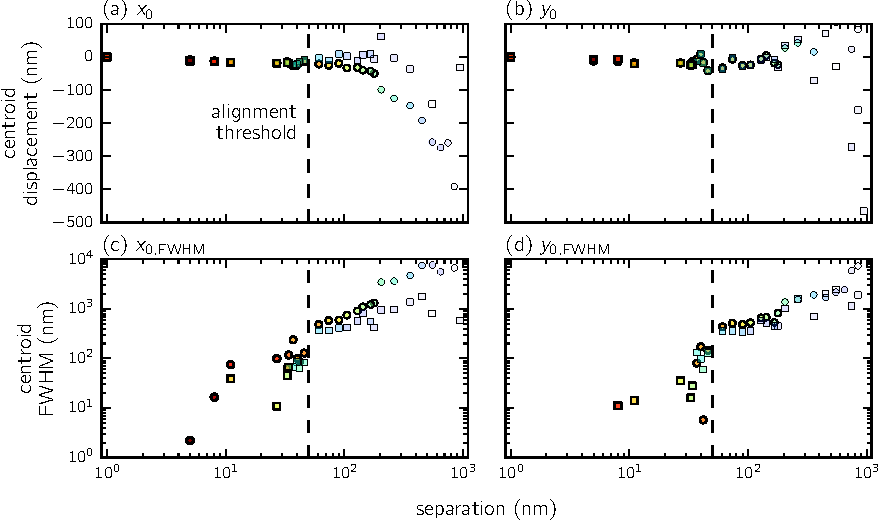
\includegraphics{figures/centroid_tracking}
\caption[Centroid tracking during approach and alignment of two sharp Au tips]{\textbf{Centroid tracking during approach and alignment of two sharp Au tips.} Amplitude (circles) and phase (squares) centroid positions relative to final alignment are shown in both the $x$ (a) and $y$ (b) directions. The centroid FWHM for the $x$ and $y$ amplitude and phase centroids are shown in (c) and (d), respectively. Marker colours indicate the strength of the peak in each alignment scan. A voltage of \SI{8}{V} was maintained during each scan. The final separation is an order of magnitude estimate based on the eventual snap-in point and the onset of the tapping mode.}
\label{fig:centroid_tracking}
\end{figure}
The centroids as a function of separation for a representative scan are shown in \autoref{fig:centroid_tracking}.

Alignment is classified as the point at which the amplitude centroid is in agreement with the phase centroid. This criterion is chosen since the emergence of a peak in the phase signifies that the apex-apex capacitance dominates the response and because phase centroid does not deviate significantly from its initial position (\figurename~\ref{fig:centroid_tracking}a,b). The amplitude centroid, on the other hand, follows the point of maximum capacitive coupling, which depends on the overall tip and cantilever shape, the separation regime and the driving voltage. For example, most pyramidal AFM tips are asymmetric in one direction with different opening angles from the apex, hence the point of maximum capacitance occurs when the higher angle tip facets overlap. As the separation decreases the apex-apex capacitance begins to dominate since the relative capacitance contributions to the amplitude go as $d^{-2}$, hence the fractional change in the intertip separation is far greater than the fractional change in the cantilever separation. Upon surpassing this point the asymmetry is effectively removed, as shown in \figurename~\ref{fig:centroid_tracking}a,b.

The accuracy of the alignment can be quantified from the FWHM of both the amplitude and phase peaks. The FWHM of both centroids shortly after passing the alignment threshold constrict to a similar length. This is inevitably limited by the feature size of the tip apex, such as the radius of a sharp or spherical tip apex. When studying spherical tips with \SI{150}{nm} radii the FWHM remains much larger since the surfaces in close proximity are much flatter in comparison. As the FWHM reduces the uncertainty on the centroid position reduces down to a few nanometres, well within the tolerance levels of any dual tip experiment.

\begin{figure}[bt]
\centering
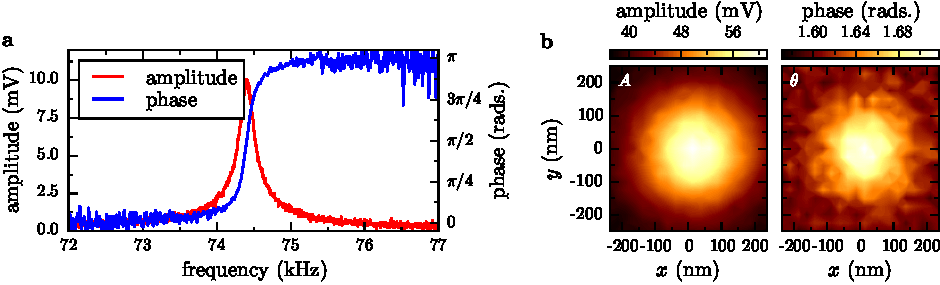
\includegraphics{figures/hf_alignment_data}
\caption[High frequency alignment data for a tip dimer composed of two \SI{48}{\newton\per\metre} Au AFM tips]{\textbf{High frequency alignment data for a tip dimer composed of two \SI{48}{\newton\per\metre} Au AFM tips.} Tips are separated by $\sim\SI{50}{nm}$ and driven at \SI{120}{V}. (a) Frequency response of the system. (b) Amplitude and phase alignment scans showing the expected peaks as the moving tip scans over the stationary tip.}
\label{fig:hf_alignment_data} 
\end{figure}

%Alignment Capabilities and Limitations
Alignment using this technique is limited to conductive tips for best results. Tips necessarily have to be conductive to generate a strong capacitive signal at the tip junction. Most tips used with this technique have therefore been from Au or Pt AFM probes, though alignment of Si tips has been demonstrated at higher voltages since they are doped to dissipate static charge. Due to the improved signal quality when using optical detection compared to electronics, smaller oscillations can be used to align tips, which is good to maintain accuracy of alignment and reduce the risk of damaging tips. For a standard sharp Au tip dimer (one contact, one tapping mode cantilever) alignment has been carried out at voltages as low as \SI{2}{V} for small tip separations. The PSD also offers at \SI{400}{kHz} bandwidth compared with the \SI{100}{kHz} bandwidth of available electronic lock-in amplifiers, allowing stiffer tips to be aligned on the occasion where a stiff dimer is needed. A demonstration of this high frequency alignment is shown in \figurename~\ref{fig:hf_alignment_data} where a large voltage of \SI{100}{V} was used to induce a sufficiently large oscillation for signal detection at \SI{74}{kHz}.

% Summary
To summarise, the capacitive alignment technique developed by Savage \textit{et al.} \cite{savage2011} has been successfully adapted to use optical cantilever detection, as in AFMs, instead of direct electronic measurements of the tip junction. The technique is greatly improved, is less sensitive to other electronic systems integrated into the microscope, and has demonstrated the capability to align two tips to within a few nanometres of the target - less than the feature size of the tips. Both the frequency and spatial response have been studied, showing the tip separation dependence and the resulting alignment mechanism.

\end{document}